\section{Results}
\label{sec:results}

\subsection{Resumption lag}

Condition had a substantial effect on resumption lag,
$F(3, 103.4) = 27.6$, $p < .001$, $\etasq = .45$. Table~\ref{tab:stats} gives
the per-condition means with confidence intervals and the planned contrasts
against \emph{Immediate}. The ordering is \emph{Ambient} best,
then \emph{Batched}, then \emph{Silent}, then \emph{Immediate}, and every
pairwise contrast against \emph{Immediate} survives Holm correction.

\begin{table*}[t]
  \centering
  \footnotesize
  \setlength{\tabcolsep}{3.6pt}
  \caption{Outcome measures by condition. Cell entries are estimated marginal
  means with 95 percent confidence intervals. Contrast columns compare each
  condition against \emph{Immediate}; a negative difference favours the listed
  condition on lag, time, and errors, and a negative difference on mental
  demand also favours it. Effect sizes are Cohen's \cohensd{}.}
  \label{tab:stats}
  \begin{tabular}{l cccc c rr}
    \toprule
    \multirow{2}{*}{Measure}
      & \multicolumn{4}{c}{Estimated marginal mean [95\% CI]}
      & \multirow{2}{*}{Best contrast}
      & \multicolumn{2}{c}{Effect} \\
    \cmidrule(lr){2-5} \cmidrule(lr){7-8}
      & Immediate & Batched & Ambient & Silent & & $\Delta$ & \cohensd{} \\
    \midrule
    Resumption lag (s)
      & 14.2 [12.9, 15.5] & 9.4 [8.3, 10.5] & 6.9 [6.0, 7.8] & 11.6 [10.4, 12.8]
      & Ambient vs Immediate & $-7.3$ & 1.12 \\
    Completion time (min)
      & 18.7 [17.2, 20.2] & 16.4 [15.1, 17.7] & 15.8 [14.6, 17.0] & 17.9 [16.5, 19.3]
      & Ambient vs Immediate & $-2.9$ & 0.58 \\
    Reverted edits (per 100)
      & 6.8 [5.6, 8.0] & 5.1 [4.1, 6.1] & 4.4 [3.5, 5.3] & 5.9 [4.8, 7.0]
      & Ambient vs Immediate & $-2.4$ & 0.51 \\
    Mental demand (0 to 100)
      & 64.3 [59.8, 68.8] & 50.6 [46.4, 54.8] & 43.1 [39.2, 47.0] & 55.2 [50.7, 59.7]
      & Ambient vs Immediate & $-21.2$ & 0.94 \\
    \bottomrule
  \end{tabular}
\end{table*}

The \emph{Silent} result is the one worth dwelling on. A condition with no
notification at all still beats an immediate toast by 2.6~s of resumption lag,
$p = .004$. Participants in \emph{Silent} polled the status bar, which costs a
glance, but a glance they initiated themselves at a moment of their choosing.
The toast arrives at a moment of the build system's choosing, and the debrief
interviews are unanimous about which is worse.

\subsection{Distribution, not just means}

Figure~\ref{fig:lag} plots the condition means with 95 percent confidence
intervals. The intervals for \emph{Ambient} and \emph{Immediate} are far apart
relative to their widths, and the ordering is stable when the analysis is
repeated on medians, which rules out an explanation resting on a few very long
recovery episodes.

\begin{figure}[t]
  \centering
  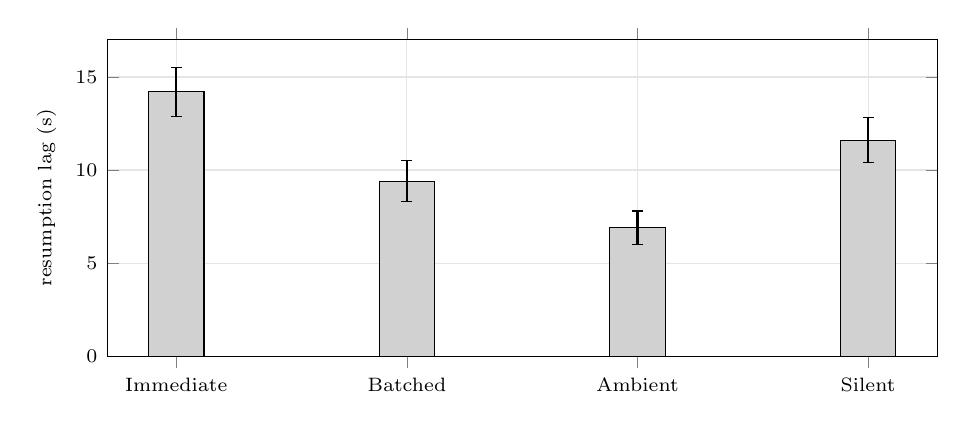
\begin{tikzpicture}
    \begin{axis}[
        width=\linewidth, height=5.6cm,
        ybar, bar width=20pt,
        ylabel={resumption lag (s)},
        symbolic x coords={Immediate, Batched, Ambient, Silent},
        xtick=data,
        xticklabel style={font=\scriptsize},
        ymin=0, ymax=17,
        grid=major, grid style={gray!20},
        tick label style={font=\scriptsize},
        label style={font=\scriptsize},
        error bars/y dir=both,
        error bars/y explicit,
        error bars/error bar style={black,thick},
      ]
      \addplot[fill=black!18,draw=black] coordinates {
        (Immediate, 14.2) +- (0, 1.3)
        (Batched,    9.4) +- (0, 1.1)
        (Ambient,    6.9) +- (0, 0.9)
        (Silent,    11.6) +- (0, 1.2)
      };
    \end{axis}
  \end{tikzpicture}
  \caption{Mean resumption lag by condition with 95 percent confidence
  intervals, $n = 36$. The ambient gutter marker halves the lag of an immediate
  toast and also improves on delivering nothing at all.}
  \label{fig:lag}
\end{figure}

\subsection{Gaze evidence for the mechanism}

The gaze traces separate the two candidate explanations. If immediate toasts
cost time because they carry more information to process, we would expect
longer dwell on the toast itself. We do not see that: mean dwell on the toast
region is 0.9~s, and mean dwell on the gutter marker is 0.4~s, a difference far
too small to account for a 7.3~s gap in resumption. What we do see is that in
the \emph{Immediate} condition the gaze leaves the primary edit region for a
mean of 5.8~s per notification, against 1.1~s in \emph{Ambient}, and that the
excess is spent reorienting after the dismissal rather than reading. The cost
is the attention shift, as~\citet{okonjo2016peripheral} would predict, not the
information.

\subsection{Order and learning effects}

Block position had no significant effect on any outcome
($p > .18$ in all four models), and adding a condition-by-position interaction
did not improve fit by likelihood ratio test, $\chi^2(9) = 11.2$, $p = .26$.
Participants did not adapt to the immediate toast over a session, which is
consistent with the field observation that developers who have used such tools
for years still report them as disruptive~\citep{steinbach2019telemetry}.
